% ****** Start of file aipsamp.tex ******
%
%   This file is part of the AIP files in the AIP distribution for REVTeX 4.
%   Version 4.1 of REVTeX, October 2009
%
%   Copyright (c) 2009 American Institute of Physics.
%
%   See the AIP README file for restrictions and more information.
%
% TeX'ing this file requires that you have AMS-LaTeX 2.0 installed
% as well as the rest of the prerequisites for REVTeX 4.1
%
% It also requires running BibTeX. The commands are as follows:
%
%  1)  latex  aipsamp
%  2)  bibtex aipsamp
%  3)  latex  aipsamp
%  4)  latex  aipsamp
%
% Use this file as a source of example code for your aip document.
% Use the file aiptemplate.tex as a template for your document.
\documentclass[%
notitlepage,
 %reprint,%
%author-year,%
%author-numerical,%
%draft,
]{revtex4-1}

\usepackage{graphicx}% Include figure files
\usepackage{dcolumn}% Align table columns on decimal point
\usepackage{bm}% bold math

% packages added by Anand
\usepackage{subfig}
\usepackage{color}
\usepackage{amsmath}
\usepackage{amssymb}
\usepackage{xspace}
\usepackage{multirow}
\usepackage{bm}
%\usepackage[mathlines]{lineno}% Enable numbering of text and display math
%\linenumbers\relax % Commence numbering lines
\include{custom_commands}
\everymath{\displaystyle}

\newcommand{\pd}[2]{\frac{\partial #1}{\partial #2}}
\newcommand{\be}{\ensuremath{{\beta}}\xspace}
\newcommand{\ret}{\ensuremath{ Re_{\theta} \xspace}}
\renewcommand{\bm}{\ensuremath{{\boldsymbol\beta_{MAP}}}\xspace}
\newcommand{\mat}[1]{{\ensuremath{\bf{ #1}}}}
% comment the following lines to see figures
%\usepackage{ifdraft}
%\ifdraft{\renewcommand{\includegraphics}{\relax}}{\relax}
%\renewcommand{\includegraphics}[2][]{}
%\renewcommand{\subfloat}[0]{}
\usepackage{url}

\begin{document}

\preprint{}

\title[]{One Dimensional Problems}% Force line breaks with \\
%\thanks{Footnote to title of article.}

%\author{Anand Pratap Singh}
%\email{anandps@umich.edu}
%\affiliation{Department of Aerospace Engineering, University of Michigan, Ann Arbor, MI 48109, USA}%

\date{\today}% It is always \today, today,
             %  but any date may be explicitly specified

\begin{abstract}

\end{abstract}

%\pacs{Valid PACS appear here}% PACS, the Physics and Astronomy
                             % Classification Scheme.
%\keywords{Suggested keywords}%Use showkeys class option if keyword
                              %display desired
\maketitle
\tableofcontents
\vspace{1cm}
\texttt{code: https://github.com/anandpratap/microstructures\_1d (private repository)\\
** utilizes symbolic differentiation to generate sigma and beta, all it needs is the expression for energy function and a function for boundary conditions. Can solve for arbitrarily complex energy function.}
\section{Introduction}
The governing equation in one dimension is given by,
\begin{eqnarray}
  \sigma_x - \beta_{xx} = 0,\label{eq:main}
\end{eqnarray} 
where,
\begin{eqnarray}
  \sigma &=& \frac{\partial W }{ \partial \epsilon},\\
  \beta &=& \frac{\partial W}{\partial \epsilon_x},
\end{eqnarray}
where, $W$ is the strain energy density and $\epsilon$ is the strain. The governing equation is solved for: (i) a convex energy function which results in a linear relationship; and (ii) a non--convex energy function which leads to non--linear equation resulting in micro-structures. Inverse problem is solved for the linear case to build the energy density function from the displacement field. For the non linear case, the solution contains multiple bifurcation points in the parameter space and thus needs better strategy for inversion. 

\section{Convex Energy Function \texttt{examples/linear\_01}}
The equation for the energy function is given by
\begin{eqnarray}
  W(\epsilon, \epsilon_x) = \frac{1}{2}\mu\epsilon^2 + \frac{1}{2}\mu l^2 \epsilon_x^2.
\end{eqnarray}
Following boundary conditions are imposed on the displacement field:
\begin{eqnarray}
  u_x = 0 &&\text{ at x = 0 and L},\\
  u = 0 &&\text{ at x = 0},\\
 -\mu l^2 u_{xxx} = t &&\text{ at x = L }.
\end{eqnarray}
\begin{figure}[!h]
	\subfloat[Solution]{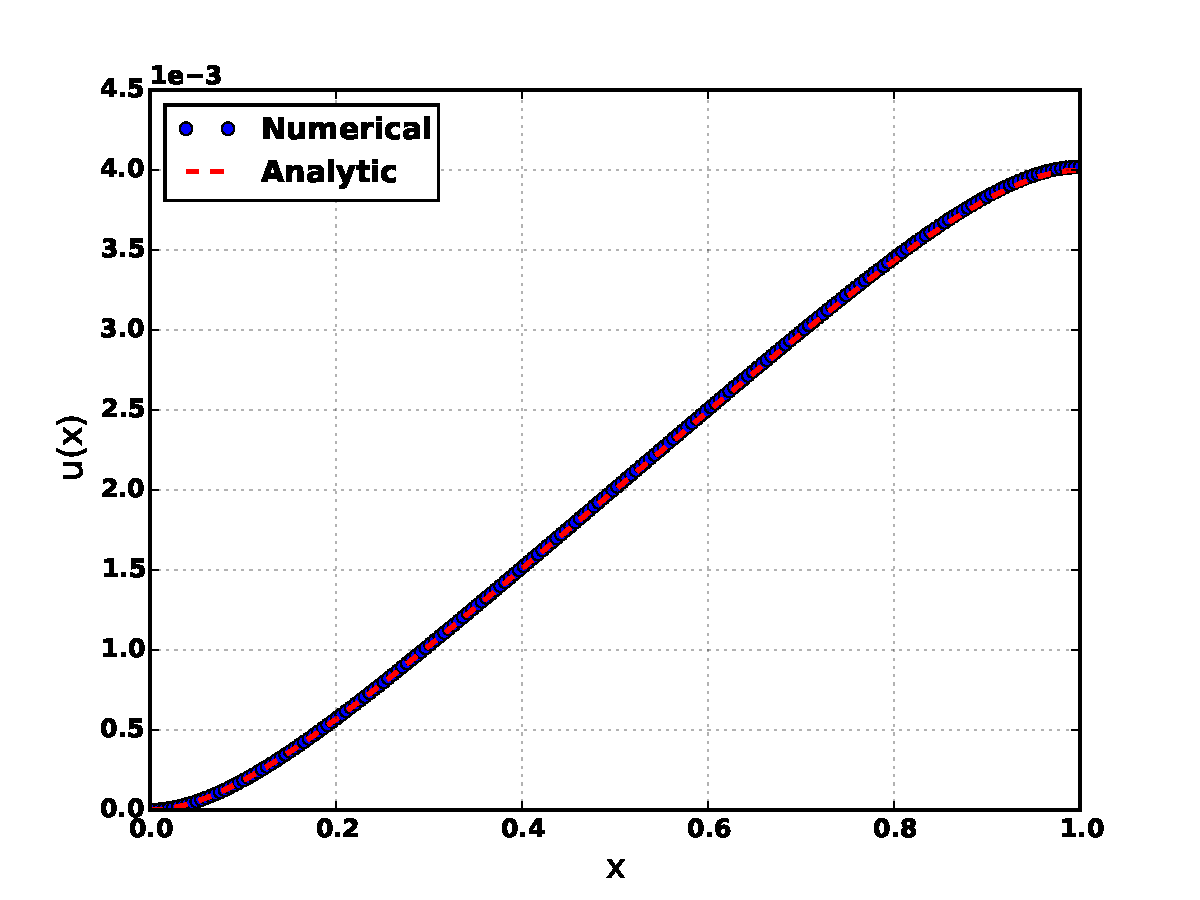
\includegraphics[width=0.45\textwidth]{figures/linear_01/solution.pdf}}
    \subfloat[Difference between the finite difference derivative and the adjoint derivative]{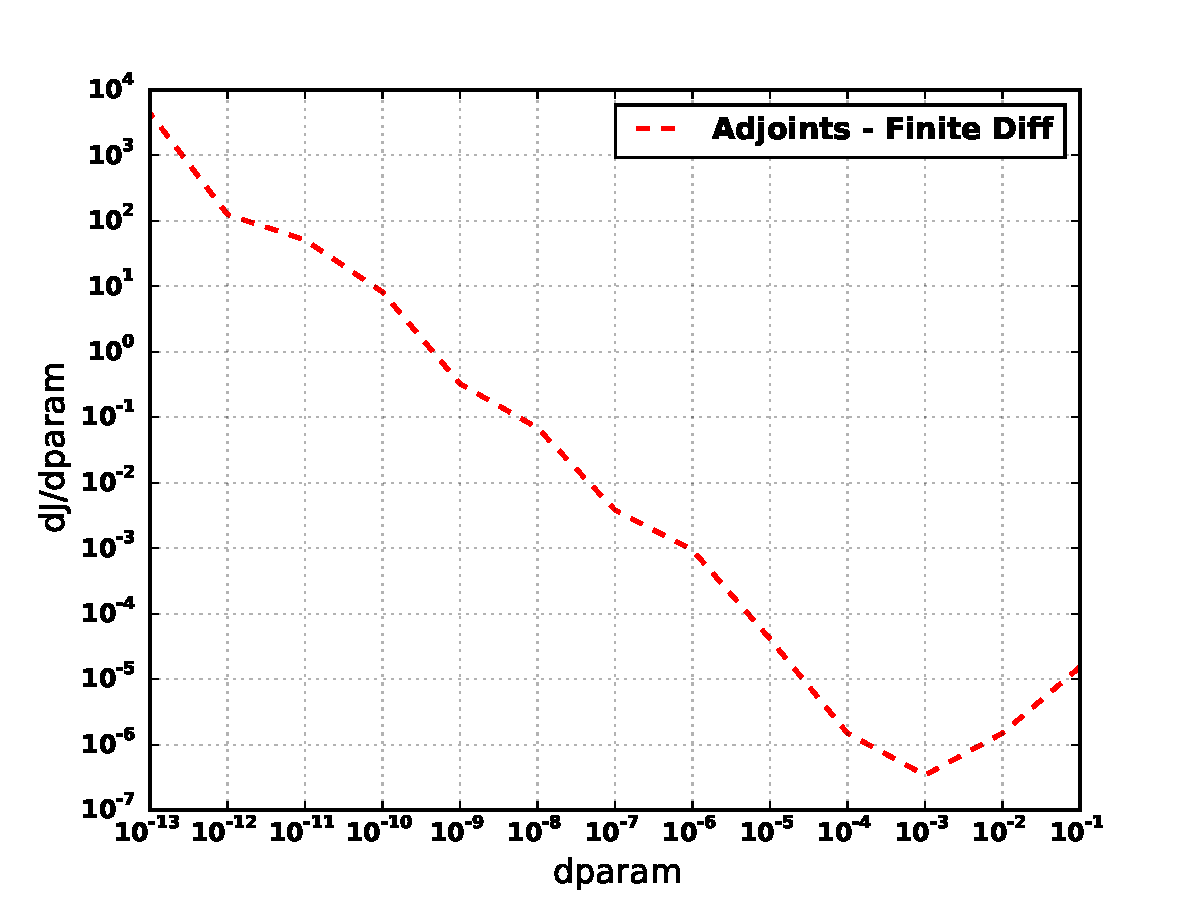
\includegraphics[width=0.45\textwidth]{figures/linear_01/sensitivity.pdf}}
    \caption{Convex energy function}
    \label{fig:convex:1}
\end{figure}
For this work, I use $\mu = 1.0$, $l = 0.1$, $L = 1$, and $t = 0.005$. The governing equation is solved using a second order finite difference scheme (refer appendix for details). A uniform grid with 200 points is used. Fig. \ref{fig:convex:1}a shows the finite difference and the analytic solution. Sensitivities are required for an inversion process, which are calculated using discrete adjoints (refer appendix for details). The difference between the sensitivities from the adjoint and the finite difference is shown in figure \ref{fig:convex:1}b. For this case, the parameter \be is the multiplier of the length scale l (i.e. $l_{effective} = \be l$) and the following objective function is used:
\begin{eqnarray}
  \mathfrak{J} = 10^4\left(\sum_j u_j^2\right) + \be^2.
\end{eqnarray}

\section{Nonlinear \texttt{examples/nonlinear\_02}}
For this case the following energy function is used:
\begin{eqnarray}
  W(\epsilon, \epsilon_x) = \frac{\mu}{\alpha^4}(\epsilon^4 - 2\alpha^2\epsilon^2) + \frac{1}{2}\mu l^2 \epsilon_x^2.
\end{eqnarray}
At the boundaries, the displacement field satisfies the following relations:
\begin{eqnarray}
  u_x = 0 &&\text{ at x = 0 and L}\\
  u = 0 &&\text{ at x = 0}\\
  u = g &&\text{ at x = L }
\end{eqnarray}
 I use $\mu = 1.0$, $g = 2^{-12}$, $l = 1/8$, $\alpha = 1/4$. Problem setup is same as in the previous case. Fig. \ref{fig:nonconvex:1} shows the solution and difference between the adjoint and the finite difference sensitivity.
\begin{figure}[!h]
	\subfloat[Solution]{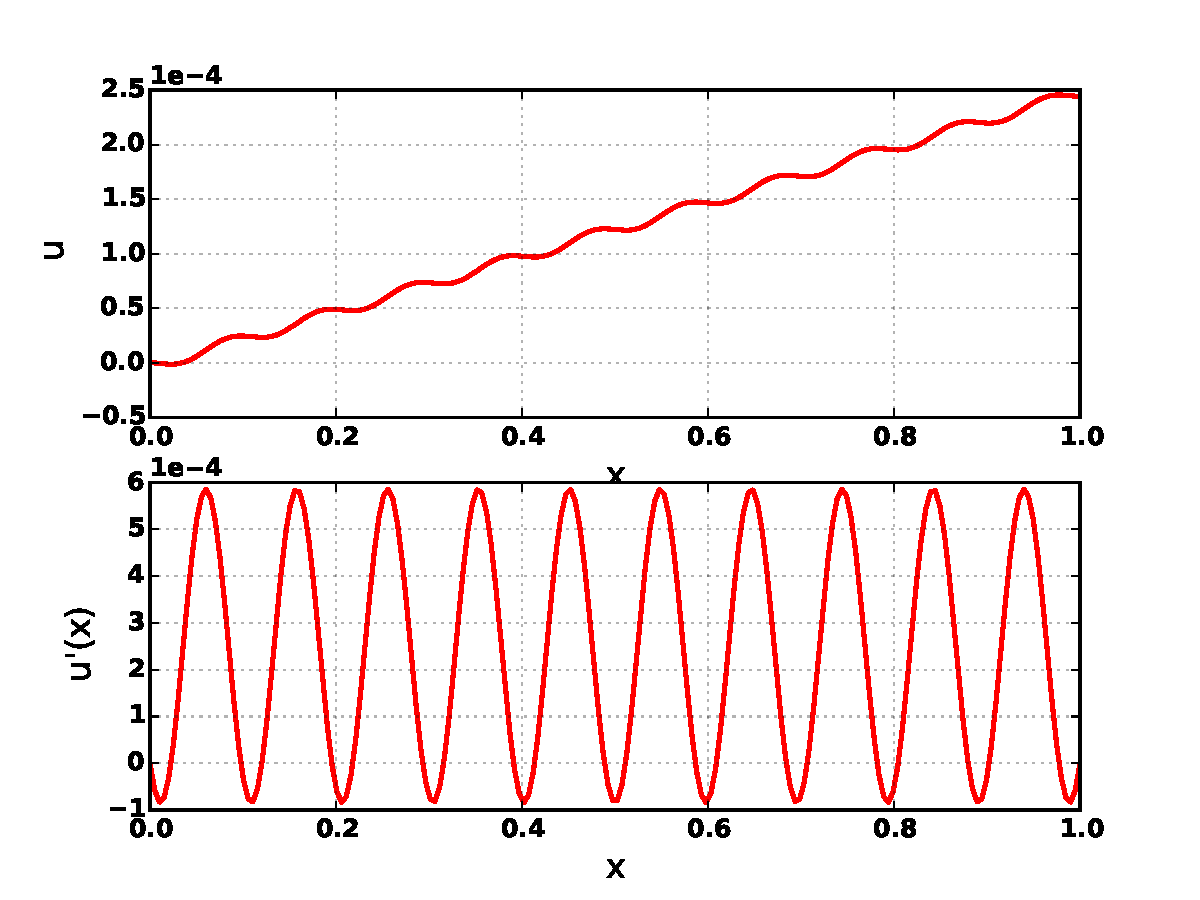
\includegraphics[width=0.45\textwidth]{figures/nonlinear_02/solution.pdf}}
    \subfloat[Difference between the finite difference derivative and the adjoint derivative]{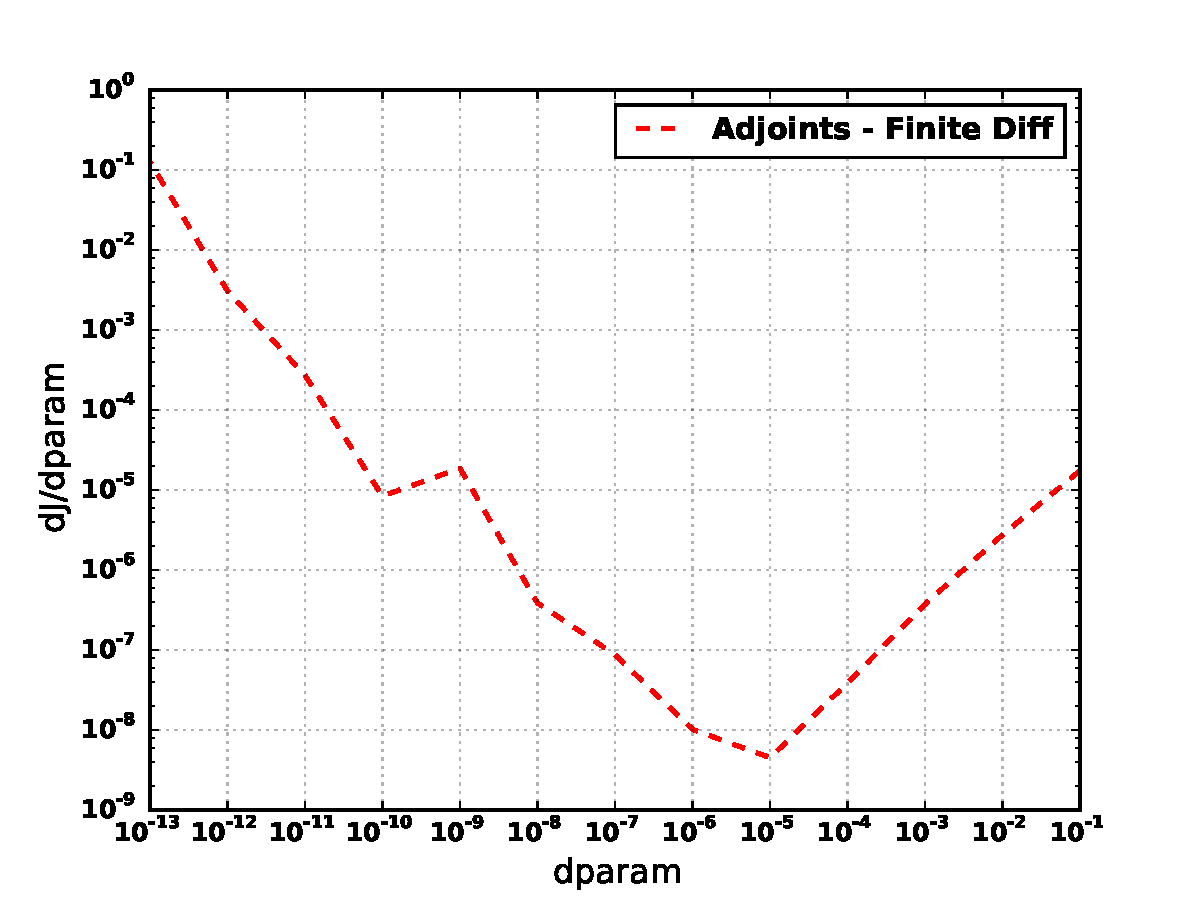
\includegraphics[width=0.45\textwidth]{figures/nonlinear_02/sensitivity.pdf}}
    \caption{Non Convex energy function}
    \label{fig:nonconvex:1}
\end{figure}
\section{Convex Inversion \texttt{examples/linear\_inverse\_03}}
This section demonstrates a simple inversion test case applied to the system with a convex energy function. The benchmark data is generated using $l = 0.1$. Starting from $l = 0.01$ -- the prior model -- the following objective function is minimized:
\begin{eqnarray}
  \mathfrak{J} = \frac{1}{2\sigma_{obs}^2}\sum_{j}(u_j - u_{obs,j})^2 + \frac{1}{2\sigma_{prior}^2}(l - l_{prior})^2
\end{eqnarray}
where $\sigma_{obs}$ and $\sigma_{prior}$ are the respective observational and the prior standard deviations representing the confidence. $\sigma_{obs} = 10^{-5}$ and $\sigma_{prior} = 1$ is used, the low observational standard deviation represents a high confidence in the data (in fact it should be zero as our data is exact!). A steepest descent algorithm with fixed step size is used to get the posterior model (note that the term \textit{posterior} is used in a loose sense, ideally posterior refers to the probability distribution, the solution which minimizes this objective function is called maximum a posteriori (MAP) solution). Another variation of the inversion with imperfect data is tested. Gaussian error, with standard deviation of 0.001, is introduced in the benchmark. For this variation, $\sigma_{obs}$ is set to 0.001. Figure \ref{fig:convex:inverse} shows the prior, posterior and benchmark data, and difference between the solution. For the case with perfect data, the inversion gives $l_{posterior} = 0.1$ (exactly same as the one used for data generation) and with noisy data $l_{posterior} = 0.09$.  

\begin{figure}[!h]
	\subfloat[Inverse solution]{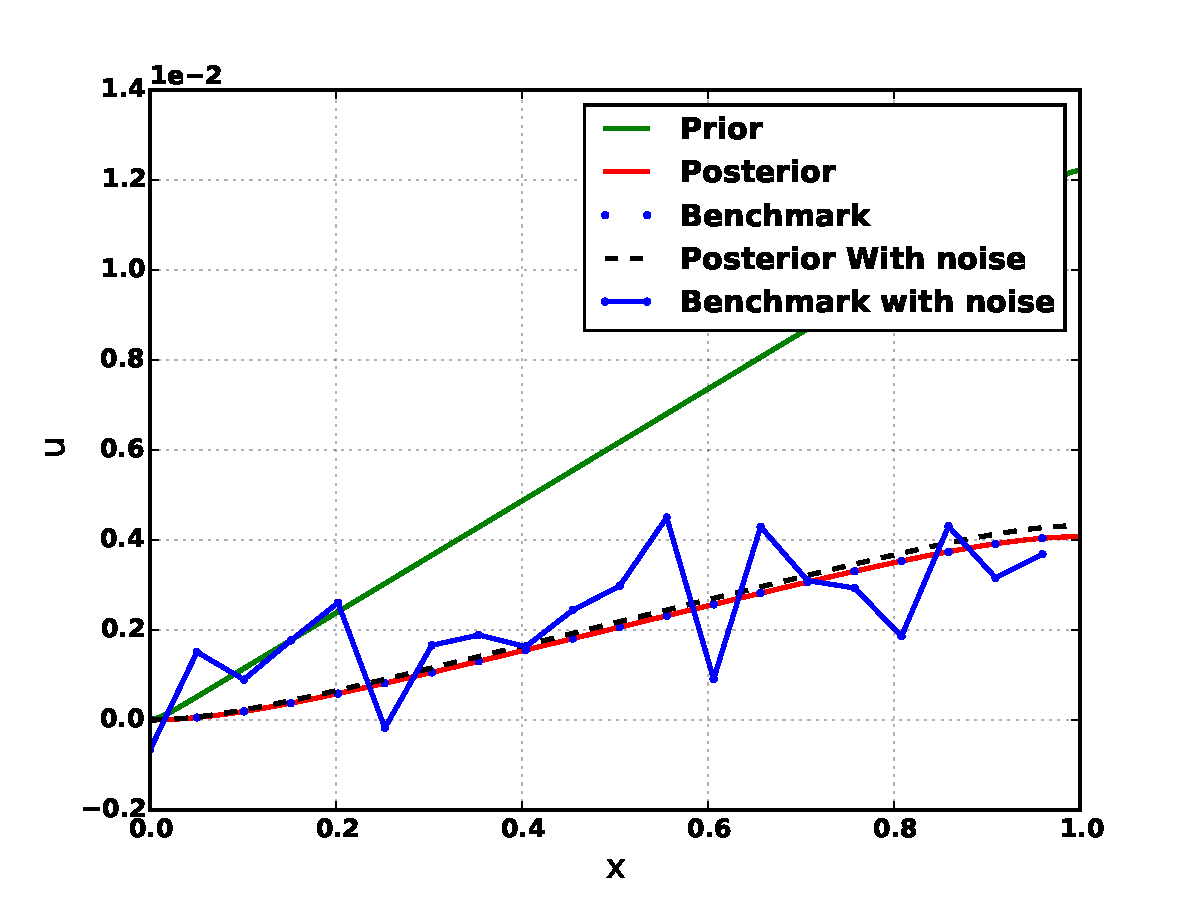
\includegraphics[width=0.45\textwidth]{figures/linear_inverse_03/inverse.pdf}}
    \subfloat[Difference between the displacement with noisy data and perfect data]{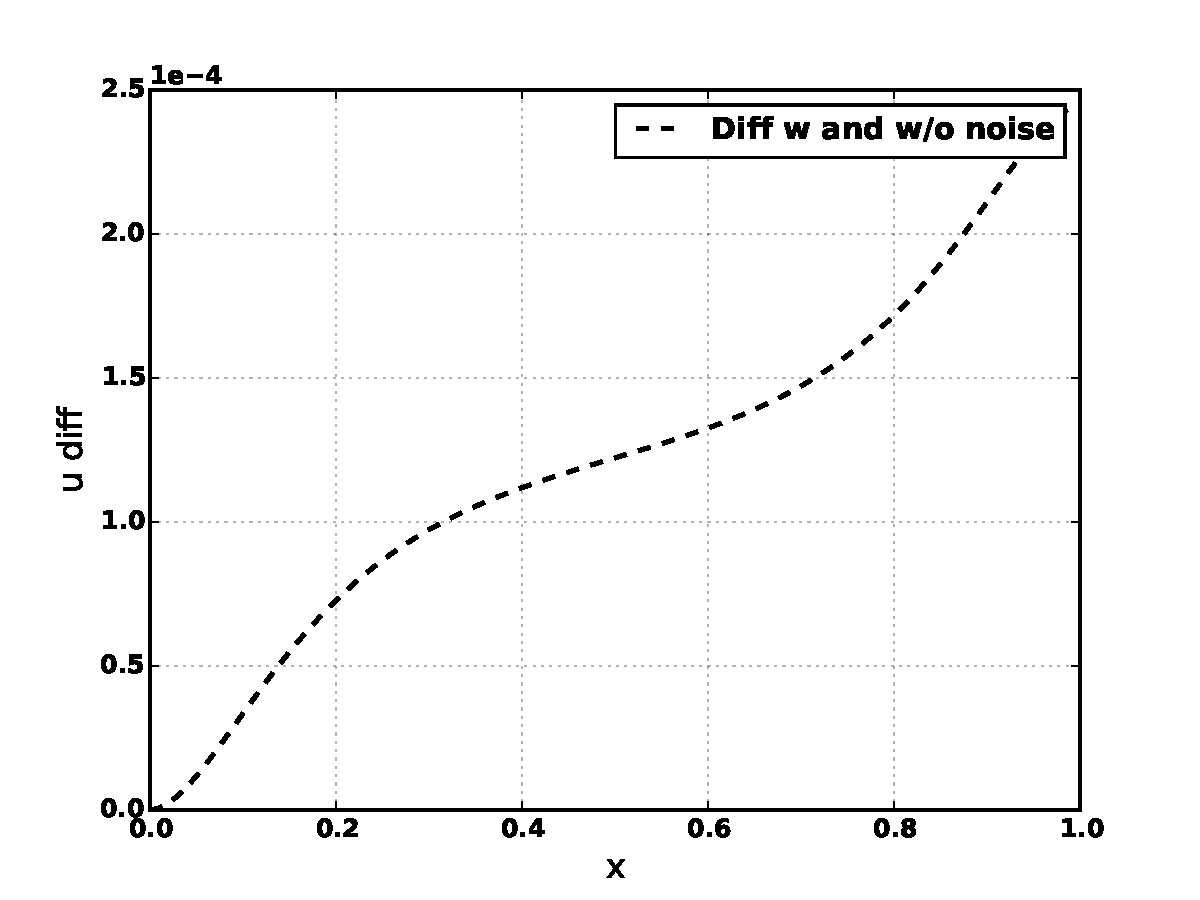
\includegraphics[width=0.45\textwidth]{figures/linear_inverse_03/diff.pdf}}
    \caption{Convex energy function inversion}
    \label{fig:convex:inverse}
\end{figure}
\section{Non convex Inversion \texttt{examples/nonlinear\_tests\_04}}
Strategy from the previous section did not work for this case. Fig. \ref{fig:nonconvex:inverse} shows the variation of the maximum value of the displacement as a function of parameter \be (hence l). Multiple bifurcation points exist for this case, therefore \textit{normal} optimization algorithms do not suffice.
\begin{figure}[!h]
	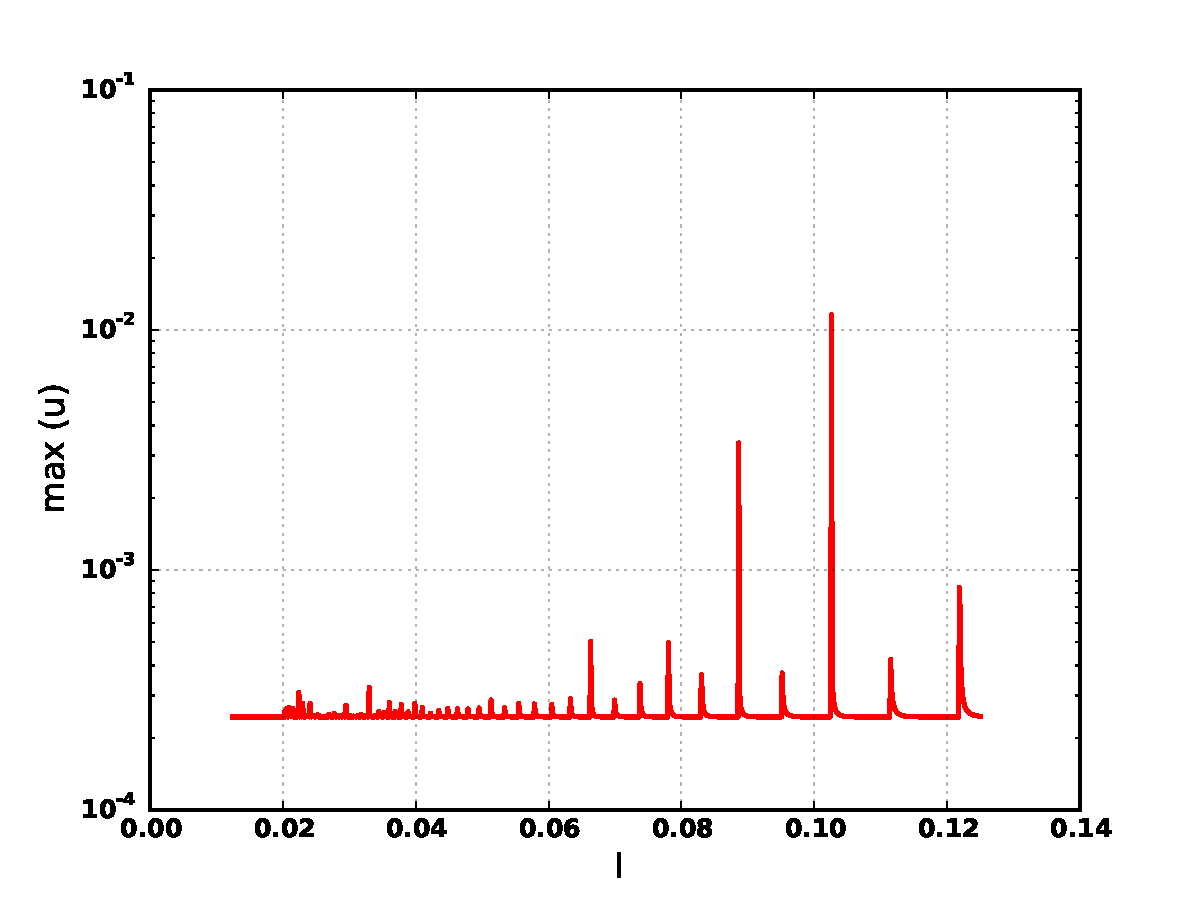
\includegraphics[width=0.85\textwidth]{figures/nonlinear_tests_04/max_u.pdf}
    \caption{Maximum displacement (max of u(x)) with variation in l (or \be)}
    \label{fig:nonconvex:inverse}
\end{figure}
\clearpage
\appendix
\section{Implementation}
Second order central difference approximation is used to discretize the derivatives at the interior points. 
\begin{eqnarray}
  u_{xxxx}(i) &=& \frac{u(i-2) - 4u(i-1) + 6u(i) - 4u(i+1) + u(i+2)}{\Delta x^4}\\
  u_{xx}(i) &=& \frac{u(i-1) - 2u(i) + u(i+1)}{\Delta x^2}\\
  u_{x}(i) &=& \frac{u(i-1) - u(i+1)}{2\Delta x}\\
\end{eqnarray}
Boundary condition at the second and the second last grid point is imposed by setting $u(i \pm 2)$ to u(i). For the first and last grid point, the residual is specified depending upon the boundary condition. For example, for the linear case,
\begin{eqnarray}
  R(1) &=& u(1),\\
  R(n) &=& - \mu l^2 u_{xxx}(i) + t, 
\end{eqnarray}
where, $u_{xxx}(i)$ is computed using one sided second order finite difference. For the non linear case, 
\begin{eqnarray}
  R(1) &=& u(1),\\
  R(n) &=& u(n) - g. 
\end{eqnarray}
Then, the problem of \mat{R}(\mat{u}) = 0 is solved using backward Euler scheme.
\begin{eqnarray}
  \Delta \mat{u} = \left(\frac{\mathbb{\mat{I}}}{dt} - \frac{ \partial \mat{R}}{ \partial \mat{u}}\right)^{-1} \mat{R}(\mat{u}^{n})\\
  \mat{u}^{n+1} = \mat{u}^{n} +  \Delta \mat{u}\\
\end{eqnarray}
The jacobian is calculated using complex step differentiation. 

Discrete adjoints are used to calculate the sensitivity of an objective function, $\mathfrak{J}$, with respect to a parameter $\be$ (it can be a vector). The total derivative with respect to \be is given by,
\begin{eqnarray}
\frac{d \mathfrak{J}}{d\be} =  \frac{\partial\mathfrak{J}}{\partial \be} + \mat{\psi}^T\frac{\partial \mat{R}}{ \partial \be},
\label{eq:appendix:1}
\end{eqnarray}
where the adjoint variable, $\mat{\psi}$, is calculated using,
\begin{eqnarray}
\left[\frac{\partial \mat{R}}{\partial \mat{{u}}}\right]^T \mat{\psi} = -\left[\frac{\partial \mathfrak{J}}{\partial \mat{{u}}}\right]^T.
\label{eq:appendix:2}
\end{eqnarray}
All the partial derivatives are calculated using complex step differentiation.
  
\end{document}

%
% ****** End of file aipsamp.tex ******
